\chapter{Introduction}
\index{Introduction@\emph{Introduction}}%

\section{Software Defined Networks}
\index{Software Defined Networks@\emph{Software Defined Networks}}%

The growth that the Internet has reached is causing several changes on the networking industry. The Internet components are reaching a limit, and thus slowing down the innovation and progress on the area. Nowadays, there is no practical method for the researchers to experiment with new network protocols in a realistic setting that will grant confidence for their widespread deployment, as a result, a lot of new ideas pass untried and untested \cite{mckeown2008openflow}.

To overcome this barrier, a joint effort of Stanford University, the University of California at Berkeley, and a number of other universities founded the Global Environment for Network Innovation (GENI) program in 2000 \cite{li2013software}.

A very important outcome of the GENI initiative is the Software Defined Networking (SDN), which was introduced on 2006 \cite{casado2006sane}. Its main goal is to evolve the vertical network model that is currently used into a more horizontal model. In the SDN model, the control plane is separated from the data plane, so that thee control plane is able to run in software on standard servers rather than in the router itself, making the switches simple forwarding devices and allowing the control logic to be logically centralized in the controller \cite{kreutz2015software}. Figure \ref{f:SDN_arch} shows a simplified view of the SDN architecture, it is important to mention that even when the controller is logically centralized, that does not means it is physically centralized, actually, in order to have the expected levels of performance, reliability and scalability is necessary to have a physically distributed control panel.


\begin{figure}[htb] % Imported eps example.
	\begin{center}
 		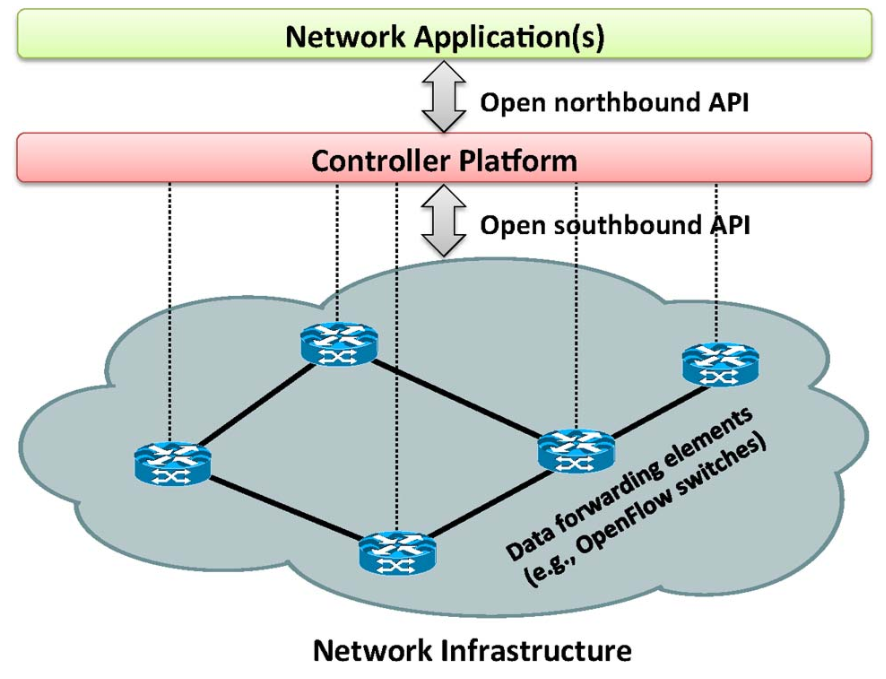
\includegraphics[width=10cm, height=10cm, keepaspectratio]{SimplifiedViewSDNArchitecture}
		\caption[Simplified View of the SDN architecture.]{Simplified View of the SDN architecture. Taken from \cite{kreutz2015software}}
		\label{f:SDN_arch}
	\end{center}
\end{figure} 


This new model of network will allow a number of new capabilities like a rapid introduction new network functions, given that the changes will be applied at software level, rather than hardware or firmware \cite{li2013software}. 

Since the goal is to apply new features to the switches it is necessary that these switches allow to be programmed. One way to do it is persuade the equipment vendors to provide and open platform on their switches that allow the researchers can experiment their new protocols, this alternative is very unlikely because vendors will not want to open up the interfaces that they have spend years developing.

Another alternative is to use existing open software platforms, but these alternatives do not have the required performance nor port density. A more promising approach is OpenFlow, which exploits the common set of functions that run in the flow-tables of many switches from different vendors, which keeps the vendors necessity for closed platforms \cite{mckeown2008openflow}.

OpenFlow provides an open protocol that allows to program the flow-tables on routers of different vendors. With this protocol, the network administrator can partition the network traffic and allow the researchers to control their own flows and their processing. This allows the research to try new routing protocols, security models and addressing schemes, all this on the same network that has an isolated traffic that is being processed with the regular schemes to avoid affectation of the network \cite{mckeown2008openflow}.

An OpenFlow switch consists of one or more flow-tables, a group-table and a secure channel to an external controller. Each of the flow-tables contains a set of flow entries, each entry consists of matching fields, counters and instructions to apply to the packet. The matching occurs in a pipeline manner through all the tables, the entries on the tables are ordered by priority, so that the first matching entry will be used. Once the match is found the actions associated are executed. If no match is found then the packet may be forwarded to the controller or dropped, depending on the switch configuration.

The entries on the flow-tables can also point to a group, which specifies an additional processing, this action groups are stored on the group-table, each of this groups contains a list of action buckets with specific semantics that depend on the group type. 

The OpenFlow channel is the interfaces that connects the switches to a controller, through this interface, the controller configures and manages the switch \cite{openflow2011openflow}.



\section{Bounded Model Checking}
\index{Bounded Model Checking@\emph{Bounded Model Checking}}%

Model Checking refers to a set of algorithms that verify the properties of state transitions systems using a search of their associated state transition graph. The properties to be verified are expressed using temporal logic, this kind of expressions allow, for example, to assert a property which is not true in the present but may eventually become true in the future \cite{clarke2001bounded}.

The model checking implementations started at the 1980s \cite{clarke1986automatic}, but these used explicit representations of state transition graphs and, with the state explosion problem where the number of states is growing exponentially, the use of these techniques is no longer possible. This techniques were used for designs with less than a million states, making them unsuitable for industrial usage. 

In the 1990s techniques that used symbolic state space exploration appeared. These techniques explore the state space through the use of Binary Decision Diagrams (BDD) \cite{burch1992symbolic}. The BDDs hold the characteristic functions of sets of states, allowing the computation of transitions among sets of states rather than individual sets. However, even though these techniques increased the order of magnitude in the size of the designs that could be verified using model checking, it was still insufficient for the industrial designs \cite{clarke2001bounded}.

A technique called bounded model checker emerged on the 2000s. This method is applicable to safety (Bad things will not happen) and liveness (Good things will eventually happen) properties. The verification of a safety property involves checking if a set of states is reachable, and the verification of liveness properties involves detecting loops in a system. This method requires little by-hand manipulation from the users, while the BDD based verification often requires manual variable ordering, or other handmade abstractions. The robustness and capacity of this method makes it a very suitable one for industrial applications.

The main disadvantage of this method is that it lacks completeness because the model is checked until a certain number of transitions have occurred, indicating errors where there are none or hiding errors that require a lot of running time. That is the reason why the main use of this tool is to find bugs, rather than proving correctness \cite{clarke2001bounded}. 


\section{SDN Verification}
\index{SDN Verification@\emph{SDN Verification}}%

Software Defined Networks have the advantage of having a logically centralized controller, this makes easier the work of programming the network and try new things on it. But since the abstraction is going to a higher level, is also more difficult to verify the correctness of the algorithm that is being used. Currently there is not much research going in that direction. 

In order to be able to verify the SDN controller we need to know which model is going to be use to describe the controller and the network, what is going to be the golden model against which the controller is going to be verified, how is the controller going to be translated a verifier input and finally, what can be verified \cite{podymov2013uppaal}. 

The most related paper that was found is from Podymov and Popesko \cite{podymov2013uppaal} where the SDN description was done using the Unified Modeling Language (UML), a modeling language for software architecture which express formal logic constraints on design elements \cite{medvidovic2002modeling}. Then, using UPPAALL \cite{larsen1997uppaal} the verification was done, comparing the UML model against formal property descriptions.

%This document deals with how to write a doctoral dissertation 
%using \LaTeX{}, and how to use the \texttt{utdiss2} package. 
%\index{utdiss2 package@{\texttt{utdiss2} package}}%
%
%The latest version of this document/package can be obtained from
%\url{http://www.ph.utexas.edu/~laser/craigs_stuff/LaTeX/}.\footnote{I
%will be transferring this page to the Office of Graduate
%Studies when I graduate. The new URL isn't defined yet, but I will
%place a ``redirect'' at this URL to send your browser to the correct
%location when the transition occurs.}
%If your installation of LaTeX is missing any style files used in this
%document (most likely with a \cn{usepackage\{package-name.sty\}}
%command at the beginning of disstemplate.tex), take a look at the link
%on this page to ``Frequently Requested Style Files'' or on the
%Comprehensive TeX Archive Network, \url{http://www.ctan.org}.
%
%In case of any confict between the requirements of the Office of Graduate
%Studies and what this document says to do, the requirements of the Office
%of Graduate Studies prevail.
%
%\section{History of This Package}
%\index{History of This Package@\emph{History of This Package}}%
%
%In 1991 the \texttt{utdiss} package was written by Young U. Ryu 
%\index{Young U. Ryu}%
%in order to be used in the preamble of \LaTeX{} doctoral dissertation
%files at the University of Texas at Austin. 
%\index{University of Texas at Austin}%
%Since then some changes have occured, the most important one
%being the introduction of a new version of \LaTeX{} 
%\index{LaTeX@{\LaTeX{}}}%
%called \LaTeXe{}. 
%\index{LaTeX2e@{\LaTeXe{}}}%
%
%In order to partially adapt the utdiss package to this new version
%of \LaTeX{}, Miguel Lerma introduced a few modifications in it,
%and his document, \textit{How to Write a Doctoral Dissertation
%with \LaTeX{}}, served as a test for it. His new package was
%called \texttt{utdiss1}.
%\index{utdiss1@\texttt{utdiss1}}%
%
%With the significant changes in style introduced by the Graduate
%School in the Spring of 2001, as well as  my need to write a
%dissertation myself, I extended Miguel Lerma's package to meet
%these new requirements. As in Miguel Lerma's case, this document
%serves as a test for it, but it is, in addition, intended as a
%template for others to use in writing their own dissertations.
%The new package is called \texttt{utdiss2}.
%\index{utdiss2@\texttt{utdiss2}}%
%
%\section{Revised Philosophy for This Package}
%\index{Revised Philosophy for This Package@\emph{Revised Philosophy
%	for This Package}}%
%
%Since the source file of this document is intended to be used by students
%writing their own dissertations, this document does not display all of the
%comments regarding usage of previous versions. It has, instead, transferred
%these comments to their respective places in the source file so someone
%editing their own copy of the source file to produce their own dissertation
%will see the comments where they are needed. It may be helpful to print out
%a copy of the source file along with the PostScript version of the document
%so the two can be studied side-by-side.
%
%\textbf{Note:} In spite of the effort to accommodate the package to
%the requirements of the University, it is not possible to guarantee
%that it will always work, and the author of the dissertation remains
%responsible for checking that such requirements are actually fulfilled
%by his/her final work. 
%
%The standard caveat applies:
%
%\begin{quote}
%\index{guarantee}%
%This template package is provided and licensed ``as is'' without warranty
%of any kind, either expressed or implied, including, but not limited to,
%the implied warranties of merchantability and fitness for a particular
%purpose. Yadda, yadda, yadda, \ldots
%\end{quote}
%
%In case of any problem with the use of \texttt{utdiss2}, send me email
%at \url{mccluskey@mail.utexas.edu}.
